

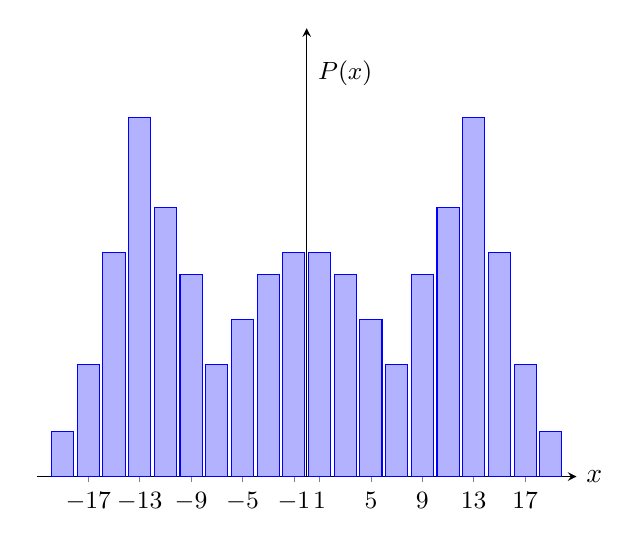
\begin{tikzpicture}
    \begin{axis}[
        ybar,
        bar width=8pt,
        ymin=0,
        ymax=10,
        xmin=-21,
        xmax=21,
        xtick={ -17, -13, -9, -5, -1, 1, 5, 9, 13, 17},
        ytick={0},
        axis x line=middle,
        axis y line=middle,
        xlabel={$x$},
        ylabel={$ $},
        xlabel style={at={(ticklabel* cs:1)}, anchor=west},
        ylabel style={at={(ticklabel* cs:1)}, anchor=south},
        every axis y label/.style={rotate=90, xshift=-0.5cm},
        yticklabel style={/pgf/number format/.cd, fixed, precision=1},
        xticklabel style={font=\small},
        bar shift=0pt,
        every axis plot/.append style={fill=cyan!70!blue}
    ]
    \addplot coordinates {
        (-19,1) (-17,2.5) (-15,5) (-13,8) (-11,6) (-9,4.5) (-7,2.5) (-5,3.5) (-3,4.5) 
        (-1,5) (1,5) (3,4.5) (5,3.5) (7,2.5) (9,4.5) (11,6) (13,8) (15,5) (17,2.5)(19,1)
    };
    \node at(3,9) {\small{$P(x)$}};
    \end{axis}
\end{tikzpicture}

